% !TEX program = lualatex
\documentclass[11pt]{article}

\usepackage[a4paper,margin=2.3cm]{geometry}
\usepackage{amsmath,amssymb,amsfonts}
\usepackage{mathtools}
\usepackage{graphicx}
\usepackage{float}
\usepackage{booktabs}
\usepackage{array}
\usepackage{caption}
\usepackage{titlesec}

% --- 字型：本文用 Noto Sans TC，英文/數學用 Latin Modern ---
\usepackage{fontspec}
\setmainfont{Latin Modern Roman}
\setsansfont{Latin Modern Sans}
\setmonofont{Latin Modern Mono}
\usepackage{luatexja-fontspec}
\setmainjfont{Noto Sans TC}
\setsansjfont{Noto Sans TC}

% --- 版面：不縮排、段距小一點，標題緊湊 ---
\setlength{\parindent}{0pt}
\setlength{\parskip}{0.45em}
\titleformat{\section}{\large\bfseries}{}{0pt}{}
\titlespacing*{\section}{0pt}{1.1em}{0.4em}
\captionsetup{font=small,labelfont=bf,skip=4pt}
\newcommand{\pd}[2]{\dfrac{\partial #1}{\partial #2}}

\begin{document}

\begin{center}
  {\Large\bfseries 生物系統建模與分析　作業五}\\[4pt]
  姓名：李傳漢\quad 學號：B11611027\quad 日期：5/28
\end{center}

\vspace{0.3em}

%==================================================================
\section{P1\quad 變異數傳播（25\%）}

用一階 Taylor 近似做 error propagation。通式（Eq.\ 9.3, p.186）：
\[
  \operatorname{var}(z)\approx\sum_i\sum_j \pd{f}{x_i}\,\pd{f}{x_j}\,\sigma_{ij}.
\]
不相關時 $\sigma_{ij}=0\ (i\neq j)$，只剩對角項；相關時要補上 cross-term
$2\,(\partial f/\partial x)(\partial f/\partial y)\,\sigma_{xy}$。下面三小題都照這個套。

\medskip
\textbf{(1)\ $z=e^{k_1 x}$}

偏微分：$\pd{z}{k_1}=x\,e^{k_1 x}$，$\pd{z}{x}=k_1\,e^{k_1 x}$。
\[
  \text{不相關：}\ \sigma_z^{2}=\bigl(k_1^{2}\sigma_x^{2}+x^{2}\sigma_{k_1}^{2}\bigr)e^{2k_1 x},
  \qquad
  \text{相關：}\ \sigma_z^{2}=\bigl(k_1^{2}\sigma_x^{2}+2k_1 x\,\sigma_{xk_1}+x^{2}\sigma_{k_1}^{2}\bigr)e^{2k_1 x}.
\]

\medskip
\textbf{(2)\ $z=k_1\cos(k_2 x)+k_3\sin(k_4 y)$（六個變數）}

偏微分：
\[
  \pd{z}{k_1}=\cos(k_2x),\quad \pd{z}{k_2}=-k_1 x\sin(k_2x),\quad \pd{z}{k_3}=\sin(k_4y),
\]
\[
  \pd{z}{k_4}=k_3 y\cos(k_4y),\quad \pd{z}{x}=-k_1k_2\sin(k_2x),\quad \pd{z}{y}=k_3k_4\cos(k_4y).
\]
不相關：
\[
  \begin{aligned}
  \sigma_z^{2}={}&\cos^{2}(k_2x)\,\sigma_{k_1}^{2}+k_1^{2}x^{2}\sin^{2}(k_2x)\,\sigma_{k_2}^{2}
      +\sin^{2}(k_4y)\,\sigma_{k_3}^{2}\\
   &+k_3^{2}y^{2}\cos^{2}(k_4y)\,\sigma_{k_4}^{2}
      +k_1^{2}k_2^{2}\sin^{2}(k_2x)\,\sigma_x^{2}
      +k_3^{2}k_4^{2}\cos^{2}(k_4y)\,\sigma_y^{2}.
  \end{aligned}
\]
如果只有 $x,y$ 相關，再加 cross-term $-2k_1k_2k_3k_4\sin(k_2x)\cos(k_4y)\,\sigma_{xy}$。

\medskip
\textbf{(3)\ $z=x^{3}y^{-3}$}

偏微分：$\pd{z}{x}=3x^{2}/y^{3}$，$\pd{z}{y}=-3x^{3}/y^{4}$。
\[
  \text{不相關：}\ \sigma_z^{2}=\frac{9x^{4}}{y^{8}}\bigl(y^{2}\sigma_x^{2}+x^{2}\sigma_y^{2}\bigr),
  \qquad
  \text{相關：}\ \sigma_z^{2}=\frac{9x^{4}}{y^{8}}\bigl(y^{2}\sigma_x^{2}+x^{2}\sigma_y^{2}-2xy\,\sigma_{xy}\bigr).
\]
寫成相對誤差比較好看：
\[
  \frac{\sigma_z}{|z|}\approx 3\sqrt{\Bigl(\tfrac{\sigma_x}{x}\Bigr)^{2}
      +\Bigl(\tfrac{\sigma_y}{y}\Bigr)^{2}
      -2\rho_{xy}\tfrac{\sigma_x}{x}\tfrac{\sigma_y}{y}}.
\]

%==================================================================
\section{P2\quad 滅絕機率 $P=(d/b)^{n}$ 的敏感度（25\%）}

模型（Eq.\ 9.4）：$P=(d/b)^{n}$。題目給 mean $d=0.8,\ b=0.9,\ n=10$，
std $\sigma=(0.157,\,0.174,\,0.69)$。deterministic 值
$P_{\text{det}}=(0.8/0.9)^{10}=0.308$。

\medskip
\textbf{(a)\ 單參數擾動敏感度}（Eq.\ 9.1，$S=(\Delta R/R_n)/(\Delta P/P_n)$，分別擾動 $\pm2\%,\pm10\%,\pm20\%$）

\begin{center}\small
\begin{tabular}{c c c c c}
\toprule
參數 & $\pm2\%$ & $\pm10\%$ & $\pm20\%$ & mean $|S|$\\
\midrule
$d$ & $(10.95,\ 9.15)$ & $(15.94,\ 6.51)$ & $(25.96,\ 4.46)$ & \textbf{12.16}\\
$b$ & $(-8.98,\ -11.19)$ & $(-6.14,\ -18.68)$ & $(-4.19,\ -41.57)$ & \textbf{15.13}\\
$n$ & $(-1.16,\ -1.19)$ & $(-1.11,\ -1.25)$ & $(-1.05,\ -1.33)$ & \textbf{1.18}\\
\bottomrule
\end{tabular}\\[2pt]
\footnotesize 每格為 $(S^{+},\,S^{-})$。
\end{center}

排序是 $|S_b|\gtrsim|S_d|\gg|S_n|$。$b$ 跟 $d$ 幾乎一樣大，下面 (b) 的 variance 分解也看到兩者佔比 50.7\% vs 49.2\%。

\medskip
\textbf{(b)\ 解析 variance}（Eq.\ 9.5，一階 Taylor）
\[
  \operatorname{var}(P)=\Bigl(\frac{n\bar d^{\,n-1}}{\bar b^{\,n}}\Bigr)^{2}\sigma_d^{2}
      +\Bigl(\frac{n\bar d^{\,n}}{\bar b^{\,n+1}}\Bigr)^{2}\sigma_b^{2}
      +\Bigl(\ln\tfrac{\bar d}{\bar b}\cdot P\Bigr)^{2}\sigma_n^{2}
  =0.7203.
\]
所以 $\sigma_P=0.849$，一階常態近似的 95\% CI $=[-1.36,\ 1.97]$。各項貢獻：

\begin{center}\small
\begin{tabular}{c c c}
\toprule
項 & var 貢獻 & 占比\\
\midrule
$d$ & $0.365$ & $50.7\%$\\
$b$ & $0.355$ & $49.2\%$\\
$n$ & $0.001$ & $0.1\%$\\
\bottomrule
\end{tabular}
\end{center}

\medskip
\textbf{(c)\ Monte Carlo}（$N=10000$，三個參數取 log-normal，拒絕 $d\ge b$ 的樣本）

mean $=0.206$，median $=0.094$，2.5--97.5\% 區間 $=[0.001,\ 0.883]$。

\medskip
\textbf{比較。}\ 兩種方法都指向 $b\sim d\gg n$。解析法因為一階 Taylor 加常態假設，CI 直接超出 $[0,1]$，機率不可能小於 0 或大於 1，所以這裡的 CI 不可信。MC 的分布是右偏、集中在小值，跟課本 Fig.\ 9.6 一致；deterministic 的 0.308 雖然落在分布裡，但 mean 和 median 都比它小，所以單看這個值沒什麼代表性。

\begin{figure}[H]
  \centering
  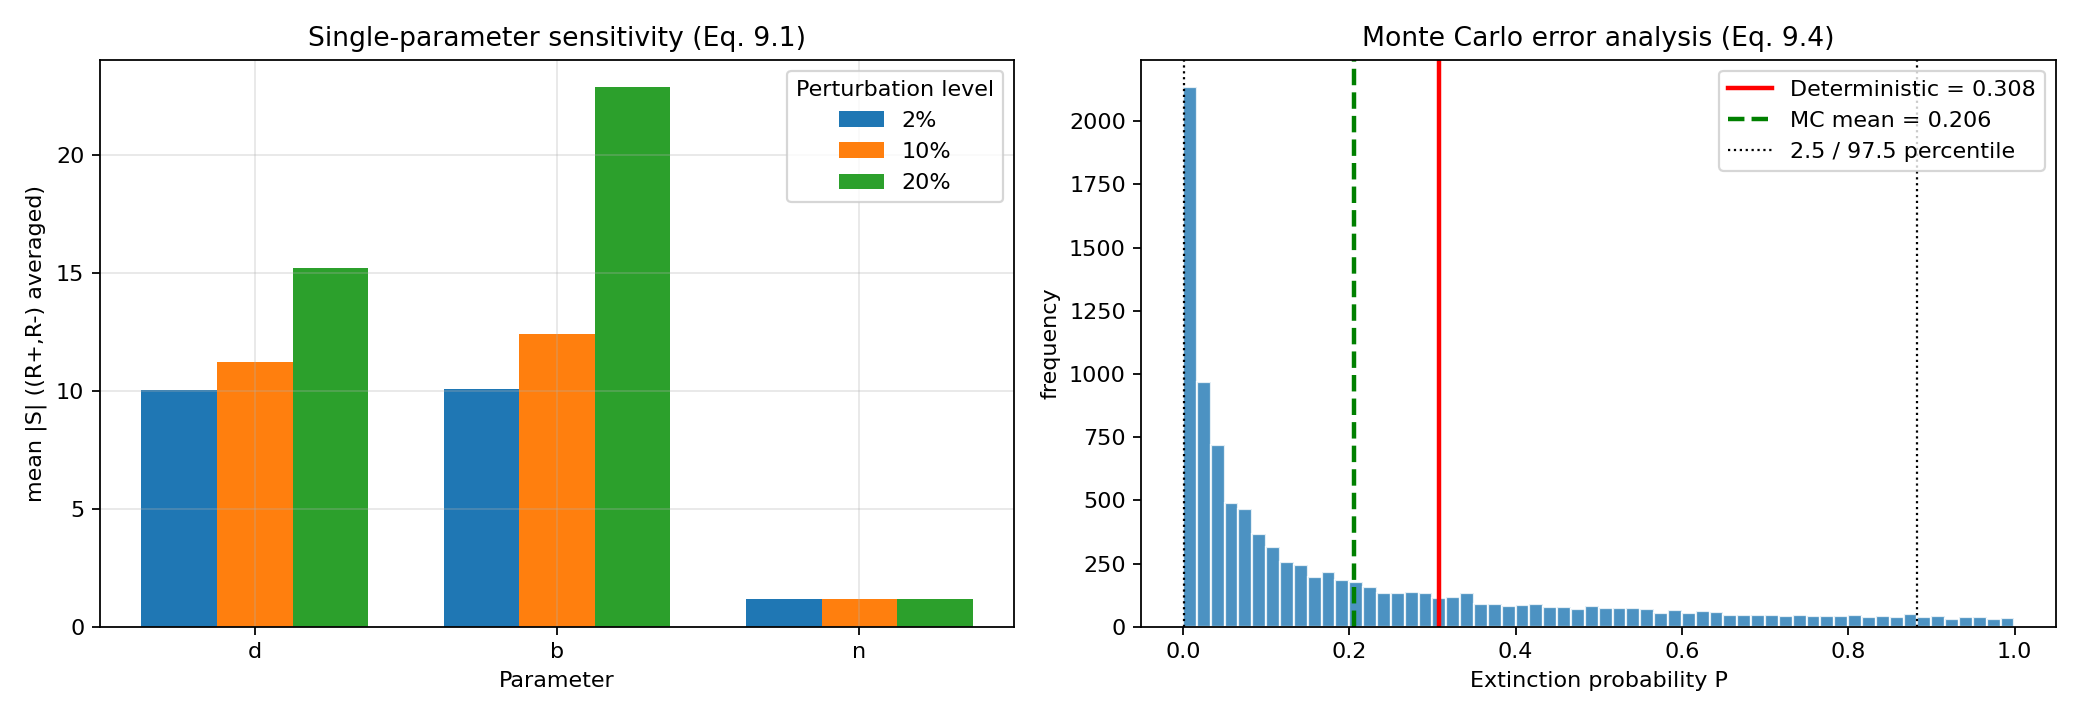
\includegraphics[width=\textwidth]{hw5_figures/fig2_problem2_sensitivity_mc.png}
  \caption{左：單參數敏感度 $|S|$，$b,d$ 遠大於 $n$。右：Monte Carlo 的 $P$ 分布；紅線為 deterministic $0.308$，綠虛線為 MC 平均 $0.206$。}
\end{figure}

%==================================================================
\section{P3\quad Gause Case III 的 local stability（25\%）}

模型（Eq.\ 9.13/9.14）：
\[
  \dot n_1=r_1 n_1\Bigl(1-\frac{n_1+\alpha n_2}{K_1}\Bigr),\qquad
  \dot n_2=r_2 n_2\Bigl(1-\frac{n_2+\beta n_1}{K_2}\Bigr).
\]
參數（除 $K_2,\beta$ 外取 p.208）：$r_1=r_2=0.05$，$\alpha=0.2$，$K_1=200$，$K_2=800$，$\beta=3$。

先確認是 Case III（Fig.\ 9.11c）：要 $K_1/\alpha>K_2$ 且 $K_1<K_2/\beta$。
這裡 $K_1/\alpha=1000>800=K_2$（成立），$K_1=200<266.7=K_2/\beta$（成立），所以確定是 Case III。

\medskip
\textbf{四個平衡點}（Eq.\ 9.17/9.18）

\begin{center}\small
\begin{tabular}{c l}
\toprule
點 & 座標\\
\midrule
$E_0$ & $(0,0)$\\
$E_1$ & $(K_1,0)=(200,0)$\\
$E_2$ & $(0,K_2)=(0,800)$\\
$E_3$ & $\Bigl(\dfrac{K_1-\alpha K_2}{1-\alpha\beta},\ \dfrac{K_2-\beta K_1}{1-\alpha\beta}\Bigr)=(100,500)$\\
\bottomrule
\end{tabular}
\end{center}

\medskip
\textbf{Jacobian}（Eq.\ 9.40）
\[
  J_{11}=r_1-\frac{2r_1 n_1}{K_1}-\frac{r_1\alpha n_2}{K_1},\quad
  J_{12}=-\frac{r_1\alpha n_1}{K_1},\quad
  J_{21}=-\frac{r_2\beta n_2}{K_2},\quad
  J_{22}=r_2-\frac{2r_2 n_2}{K_2}-\frac{r_2\beta n_1}{K_2}.
\]
代入共存點 $(100,500)$：$J_{11}=0.05-0.05-0.025=-0.025$，$J_{12}=-0.005$，
$J_{21}=-0.09375$，$J_{22}=0.05-0.0625-0.01875=-0.03125$，
\[
  J(E_3)=\begin{pmatrix}-0.025 & -0.005\\[2pt] -0.09375 & -0.03125\end{pmatrix}.
\]
特徵方程 $\lambda^{2}+0.05625\,\lambda+0.0003125=0$，
\[
  \lambda_{1,2}=\frac{-0.05625\pm\sqrt{0.05625^{2}-4(0.0003125)}}{2}
             =\frac{-0.05625\pm0.04375}{2}.
\]
\[
  \boxed{\ \lambda_1=-0.00625,\quad \lambda_2=-0.05\ \text{（兩個都負）}\ \Rightarrow\ \text{stable node}.\ }
\]

其他三個點也一起檢查：

\begin{center}\small
\begin{tabular}{c l c}
\toprule
點 & $\lambda_{1,2}$ & 類型\\
\midrule
$(0,0)$ & $(+0.05,\ +0.05)$ & unstable node\\
$(200,0)$ & $(-0.05,\ +0.0125)$ & saddle\\
$(0,800)$ & $(+0.01,\ -0.05)$ & saddle\\
$(100,500)$ & $(-0.05,\ -0.00625)$ & stable node\\
\bottomrule
\end{tabular}
\end{center}

只有共存點是穩定的，其餘三個都不穩，這跟 Case III「兩物種共存」的圖像一致。

\begin{figure}[H]
  \centering
  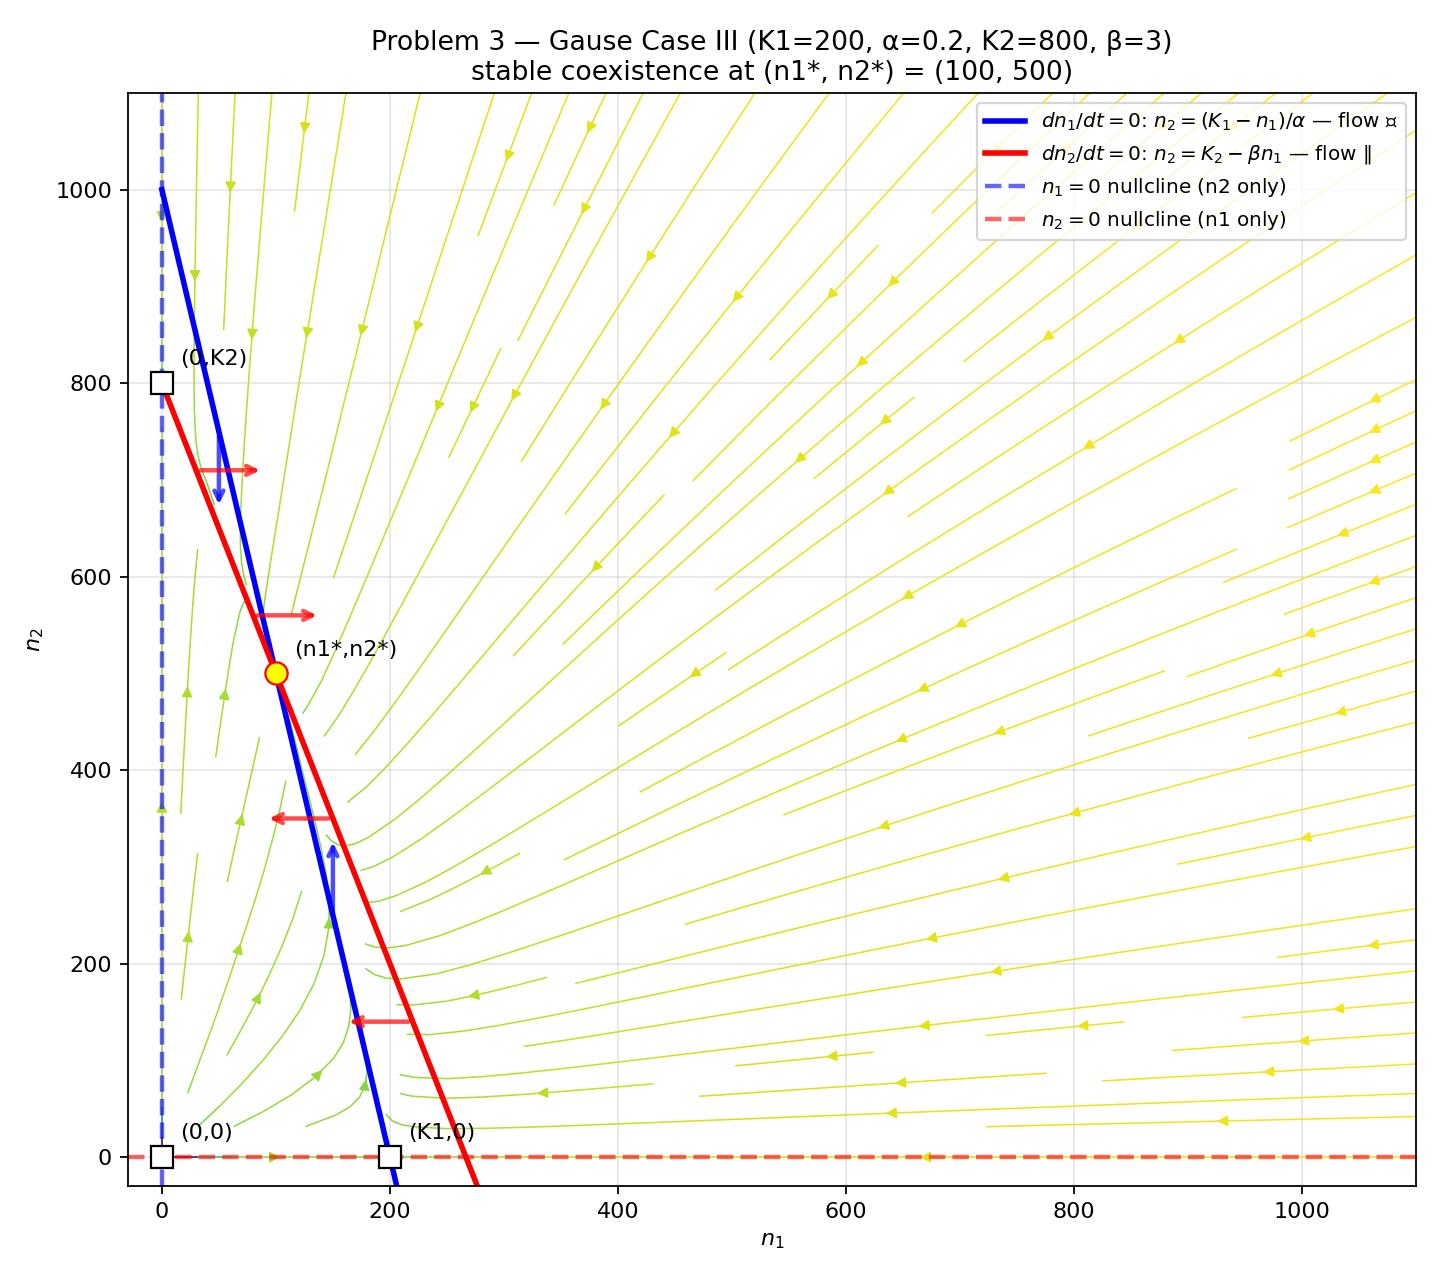
\includegraphics[width=0.62\textwidth]{hw5_figures/fig3_problem3_gause_caseIII.png}
  \caption{Case III 相圖：兩條 nullcline 交在共存點 $(100,500)$，flow field 收斂到該點。}
\end{figure}

%==================================================================
\section{P4\quad 自訂 2-D 系統的平衡點與穩定性（25\%）}

我自己設的模型：
\[
  \dot x=a_1 x^{2}-a_2 x^{3}-b\,xy,\qquad \dot y=d\,xy-f y^{2},
\]
參數 $a_1=1,\ a_2=0.05,\ b=5,\ d=1,\ f=10$。

\medskip
\textbf{(1)\ Nullclines}

\begin{center}\small
\begin{tabular}{l l l}
\toprule
nullcline & 方程 & 另一分量方向\\
\midrule
$\dot x=0$ & $x=0$（$y$ 軸） & $\dot y=-fy^{2}<0$，向下\\
$\dot x=0$ & $y=(a_1 x-a_2 x^{2})/b$（拋物線） & $\dot y=0.1xy(x-10)$；$x<10$ 向下、$x>10$ 向上\\
$\dot y=0$ & $y=0$（$x$ 軸） & $\dot x=x^{2}(a_1-a_2 x)$；$x<20$ 向右、$x>20$ 向左\\
$\dot y=0$ & $y=dx/f=x/10$（過原點直線） & $\dot x=0.05x^{2}(10-x)$；$x<10$ 向右、$x>10$ 向左\\
\bottomrule
\end{tabular}
\end{center}

\medskip
\textbf{(2)\ 平衡點}（先解符號再代數值）
\[
  E_0=(0,0),\qquad E_1=\Bigl(\frac{a_1}{a_2},\,0\Bigr),\qquad
  E_2=\Bigl(\frac{a_1 f-bd}{a_2 f},\ \frac{d(a_1 f-bd)}{a_2 f^{2}}\Bigr).
\]
代數值：$E_0=(0,0)$，$E_1=(20,0)$，$E_2=(10,1)$。

\medskip
\textbf{(3)\ Jacobian}
\[
  J=\begin{pmatrix} 2a_1 x-3a_2 x^{2}-by & -bx\\[2pt] dy & dx-2fy\end{pmatrix}.
\]
\begin{itemize}\setlength{\itemsep}{2pt}
  \item $E_0=(0,0)$：$J=\mathbf 0$，linearization 失效（degenerate），要看高階項。
  \item $E_1=(20,0)$：$J=\begin{pmatrix}-20 & -100\\ 0 & 20\end{pmatrix}$，上三角，$\lambda=(-20,\,20)$，$\det=-400<0$，是 saddle。
  \item $E_2=(10,1)$：$J=\begin{pmatrix}0 & -50\\ 1 & -10\end{pmatrix}$，$\operatorname{tr}=-10$，$\det=50$，$\operatorname{tr}^{2}-4\det=-100<0$，所以 $\lambda=-5\pm5i$，是 stable spiral。
\end{itemize}

\medskip
\textbf{(4)\ 穩定 / 不穩定的理由}
\begin{itemize}\setlength{\itemsep}{2pt}
  \item $E_2=(10,1)$ 是 stable spiral：$\operatorname{Re}\lambda=-5<0$，由 Hartman--Grobman，局部跟線性化拓樸等價，所以軌跡會螺旋收斂進去，旋轉週期約 $T=2\pi/5\approx1.26$。
  \item $E_1=(20,0)$ 是 saddle：兩個 eigenvalue 一正一負，沿 $\lambda=+20$ 對應的方向會被推開，所以不穩定。
  \item $E_0=(0,0)$ 是 degenerate：Jacobian 全 0，線性化看不出來；改看主導的高階項 $\dot x\approx a_1 x^{2}>0$，代表 $x$ 會自己離開原點，所以原點不是吸引子。
\end{itemize}

\begin{figure}[H]
  \centering
  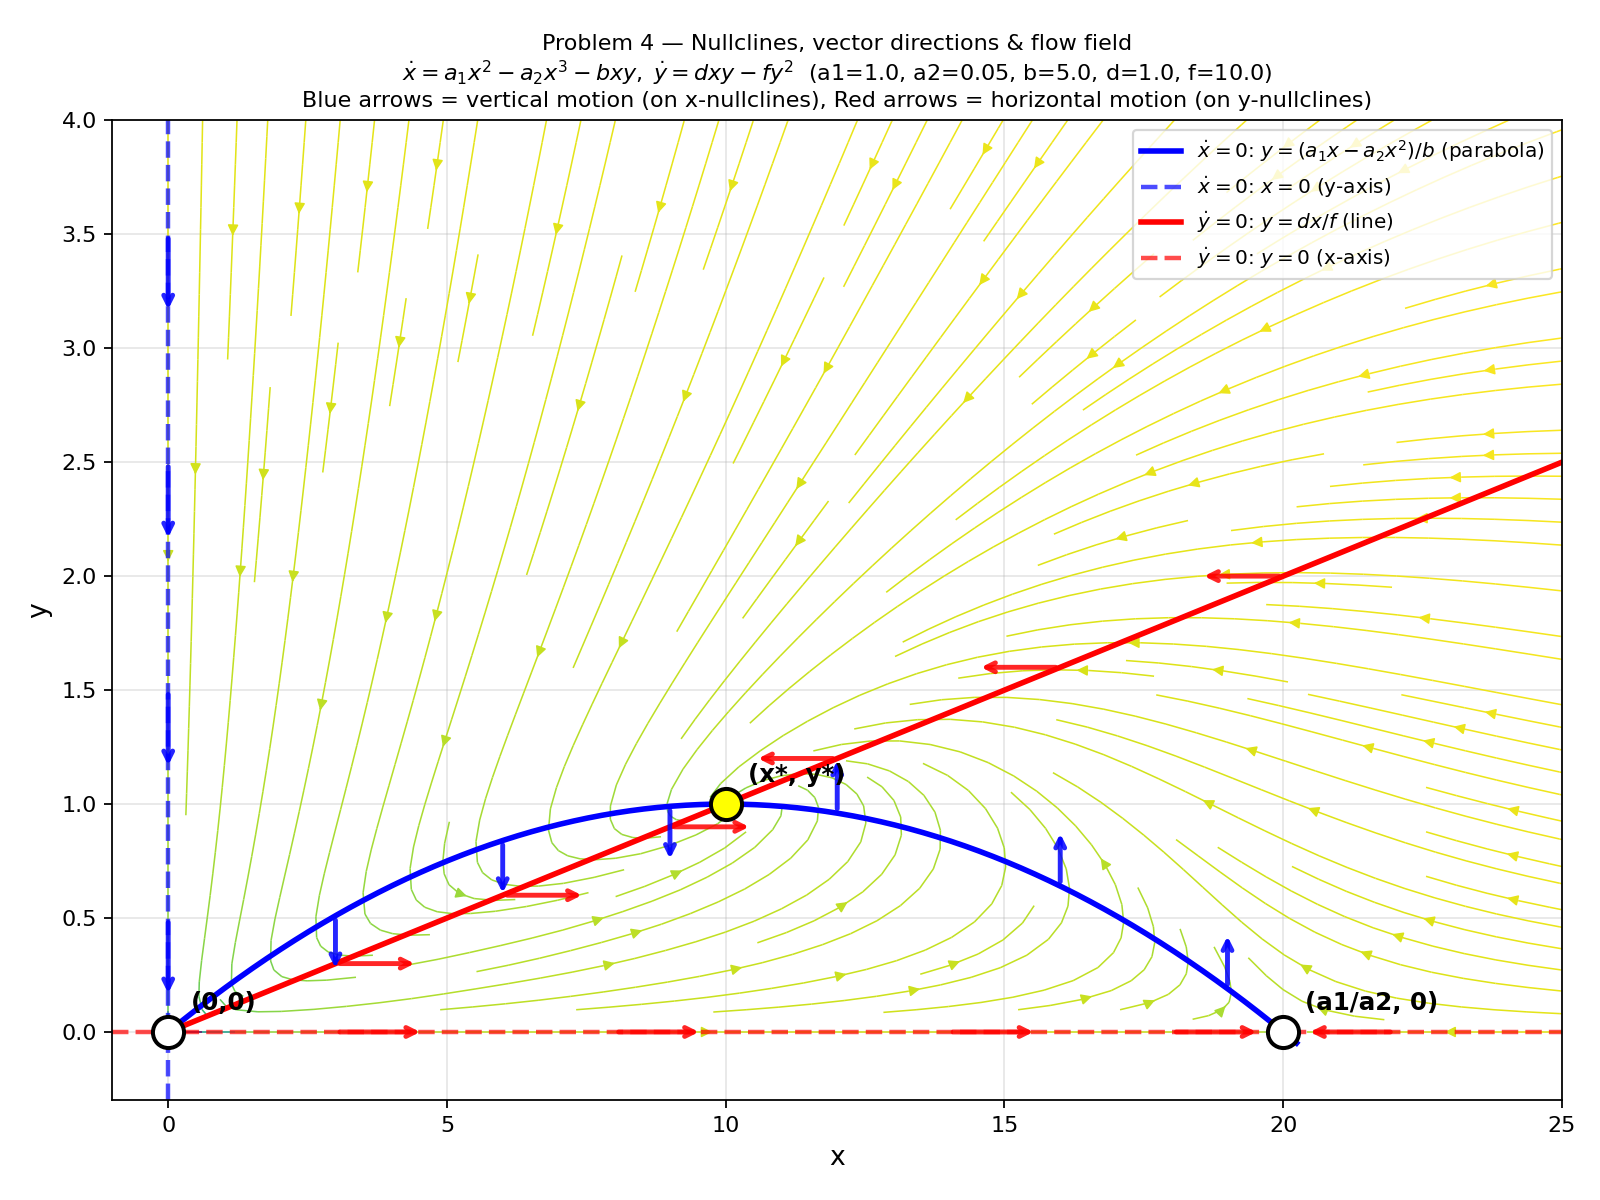
\includegraphics[width=0.72\textwidth]{hw5_figures/fig4_problem4_nullclines.png}
  \caption{P4 的 nullclines 與 flow field：$E_2=(10,1)$ 為 stable spiral，$E_1=(20,0)$ 為 saddle，$E_0$ 為 degenerate。}
\end{figure}

%==================================================================
\section*{摘要}

\begin{center}\small
\begin{tabular}{c l l}
\toprule
題 & 結論 & 關鍵數字\\
\midrule
P1 & 用 Eq.\ 9.3 一階近似推三組 var；相關時多 cross-term & ---\\
P2 & 敏感度 $b\gtrsim d\gg n$；解析 $\operatorname{var}(P)=0.72$ 但 CI 失控，MC 重現 Fig.\ 9.6 & $|S_b|{=}15,\ |S_d|{=}12,\ |S_n|{=}1$\\
P3 & Case III 共存點 $(100,500)$ stable，其餘是 saddle / unstable & $\lambda=(-0.05,\,-0.006)$\\
P4 & $E_2=(10,1)$ stable spiral；$E_1$ saddle；$E_0$ degenerate & $\lambda(E_2)=-5\pm5i$\\
\bottomrule
\end{tabular}
\end{center}

\end{document}
